% https://www.springer.com/gp/computer-science/lncs/conference-proceedings-guidelines
\documentclass[runningheads]{llncs}
%
\usepackage[T1]{fontenc}
% T1 fonts will be used to generate the final print and online PDFs,
% so please use T1 fonts in your manuscript whenever possible.
% Other font encondings may result in incorrect characters.
%
\usepackage{graphicx}
\usepackage{float}
\usepackage{hyperref}
\usepackage{amsmath}
\usepackage{parselines}
\usepackage{listings}
% Used for displaying a sample figure. If possible, figure files should
% be included in EPS format.
%
% If you use the hyperref package, please uncomment the following two lines
% to display URLs in blue roman font according to Springer's eBook style:
%\usepackage{color}
%\renewcommand\UrlFont{\color{blue}\rmfamily}
%\urlstyle{rm}
%
\begin{document}
%
\title{A System Analysis to Dkron Scheduler}


%
%\titlerunning{Abbreviated paper title}
% If the paper title is too long for the running head, you can set
% an abbreviated paper title here
%
\author{Miguel Albuquerque, 1105828\inst{1}\orcidID{1105828}}
\institute{Instituto Superior Técnico, Av. Rovisco Pais 1, 1049-001 Lisboa, Portugal
\email{miguel.albuquerque@tecnico.ulisboa.pt}}
%
\maketitle              % typeset the header of the contribution
%
\begin{abstract}
Dkron is a golang written distributed cron job scheduler that is
fault-tolerant (Reliable), and allows for concurrent job execution.
In this project tools like Azure, K9, K8, K6, and Helm were used to develop a
deployment of Dkron into (azure) AKS. The Dkron cluster was subject to benchmarking
in order to extrapolate data and form conclusions on the observed system's behavior.
Failed Requests was the metric evaluated when doing fractional factorial analysis.
The factor Concurrent and the effect interaction between the factors HasOnDemandJobs,
CPU Limit, and Memory Limit, contribute to a lower request failure. All the other factors and interactions contribute
to an increase of request failure.
\end{abstract}

\par
\text{Repository: \href{https://github.com/miguel-msa/dkron-study}{github.com/miguel-msa/dkron-study}}
\par
\text{Commit hash:} \textbf{5d3aa963e662f30096d4ce818194657248701539}
\par
\text{Video link (youtube):} \textbf{https://youtu.be/SxbSg0Dx16s}



\keywords{Dkron \and Distributed \and Benchmark \and Scalability \and Consensus \and Dkron Server \ and Dkron Agent \and Raft.}
%
%
%
% %%%
% %%%


\section{Introduction}

Distributed systems, in simple terms, are a group of systems or processes that work together
for a common goal. Being distributed, some particularities need to be considered, for instance
how do they interact, and how do they agree on a decision. Agreeableness in distributed
systems is a concept of grand study, where we have examples like Paxos and Raft, being both
consensus algorithms.

A job scheduling system purpose is to automate execution of jobs, do repetitive tasks
and, when well-defined and organized, automate entire workflows. It is expected that these jobs run within defined conditions,
for instance time-based conditions. Other use cases are resource management
(e.g., scheduled to execute for off-peak hours) and avoid manual intervention.

Dkron is a distributed job scheduling system that on the surface:

\begin{enumerate}
    \item Has flexible tag-based job definition
    \item Allows for Distributed execution, where these jobs can be ran in a distributed mode. % todo: review this!
    \item Has no Single Point of Failure.
    \item Easy to deploy with built-in replicated storage (BuntDB) relying on the Raft protocol.
    \item Provides a Web-GUI for administration.
\end{enumerate}
The above characteristics, and more, are also explored in section \ref{system_description}.

When selecting the system to analyse, some of the factors driving the choice were:
\begin{enumerate}
    \item Interest in exploring \href{https://go.dev/}{Go} source code.
    \item Explore a system that is not a database.
\end{enumerate}
From the options, Dkron raised a question:
\textit{What is the performance of a scheduler, seemingly, focused on availability and reliability?}

As this is not thoroughly explored by Dkron, I got interested in this system and how it would scale
for reliability.

~\\
Ultimately, Dkron is a golang written scheduler with specific particularities for some key use-cases.
Its claims are not bold, neither on its performance, nor on how it actually does scheduling. This opens an
opportunity to not only explore something unclaimed, but also on how Dkron found the
optimal point, if exists, between performance and reliability.

\begin{figure}[h]
\centering
%\caption{dkron Logo .} \label{fig1}
\end{figure}

\section{System Description}
\label{system_description}

Further exploring Dkron's characteristics from the summary in the introduction, some of its  particularities are:
\begin{enumerate}
    \item \textbf{Concurrency:} A job can be either ran concurrently, by default,
    allowing for overlapping jobs, or forbid concurrency.
    \item \textbf{Cron spec support:} A job can be defined either by using Dkron's
    pre-defined schedules, which are more declarative, e.g., \textit{@hourly}, or using cron expression format.
    \item \textbf{Executors:} Plugins to execute the jobs, e.g., Shell to run the job in
    the current node, or HTTP to send a request.
    \item \textbf{Metrics:} Dkron can send metrics to Statsd and provide prometheus format metrics.
    \item \textbf{Job Retries:} A job can be declared to retry in case of failure.
    \item \textbf{Embedded Storage:} Dkron uses an embedded KV store based on BuntDB.
    \item \textbf{State Storage:} The scheduler state is replicated between all
    server nodes using \href{https://www.serf.io/}{Serf}.
    \item \textbf{Target nodes spec:} By default, every node will run a job, however there is
    the ability to set tags for jobs to be ran only by target nodes identified with those
    same tags.
    \item \textbf{Clustering:} Clustering in Dkron provides fault tolerance when the
    quorum is equal or higher than 3.
    \item \textbf{Leader Recovery:} Detects if the leader is missing in the work pool,
    and (usually) elects a new leader.
\end{enumerate}


Dkron has 2 kinds of nodes: Server and Agent.
Both are cluster members available to run scheduled jobs.

An agent can handle job executions, run scripts and return the resulting output to the server.

A server does everything an Agent does, plus: schedules jobs, handles data storage,
participate on leader (Raft) election, dispatches the execution of jobs either to Agents,
or other Servers.

A Dkron cluster has a leader, for Raft based distribution, which is responsible to start job execution queries in the cluster.

By default, all nodes execute each job. This can be controlled through the use of tags and
a count of target nodes having this tag. This allows to run jobs across a cluster of any size and with any
combination of machines needed.

All execution responses are gathered by the scheduler and stored in the BuntDB storage.

\begin{verbatim}
{
    "name": "job_name",
    "command": "/bin/true",
    "schedule": "@every 2m",
    "tags": {
        "my_role": "web:1"
    }
}
\end{verbatim}

Above is an example of a job that should run only on one node, in any that has the value \textit{web}
for the tag \textit{my\_role}.


% todo: make this a paragraph instead ???
\subsection{No Single Point of Failure}
By leveraging Raft consensus algorithm, this no Single Point of Failure characteristic is very relevant for systems
that, e.g., depend on other running jobs or trigger to function - the scheduler.
The System using these schedulers might be fault-tolerant, but the scheduler itself might not, making these "fault-tolerant" systems, indirectly, not as
so - Dkron fixes this problem by, as they claim, being the only existing scheduler with no SPOF.

% ? Acceptable Performance --> we'll find out on tests
Therefore, with acceptable performance, whilst providing Reliability, Dkron is an interesting solution
for use-cases that must guarantee fault-tolerance.

\section{Benchmarking}

Due to the project time constraints, an extensive literature review was not performed, however
a great portion of this project's approach, execution and reporting is done based on the acquired
knowledge in the course.

During the limited research, I could not find a convincing standard benchmark to use or be based on.
Instead, I focused on researching the particularities of Dkron and exploiting those to gather conclusions and,
admittedly, confirm some deductions I was forming throughout Dkron's design analysis.

One of the clearest characteristic for performance analysis in Dkron is its use of Raft to guarantee
reliability. This, along the fact that all the dkron cluster members of kind Server persist,
between themselves, all the job responses' logs.

~\\ Thus, the intuitive conclusion for Dkron is:
\textbf{1)} Increase Dkron Servers to improve fault-tolerance, but increases overhead,
\textbf{2)}Increase Dkron Agents to improve performance.


Nevertheless, solely increasing Agents, even with unlimited costs, is not an infinite answer.
Even more so considering that, unless the
\href{https://dkron.io/docs/usage/target-nodes-spec}{job is targeted to a set of tags},
every member in the cluster will run the job.

With very limited information on Dkron's scaling capabilities, one can assume, contention and crosstalk will increase as most systems do.
Without a formal baseline to which to compare with, I took the liberty to think about a synthetic workload
to push the limits of Dkron whilst considering the University Scalability Law and its properties.

\[
X(N) = \frac{N}{1 + \alpha (N - 1) + \beta N (N - 1)}
\]

where:
\begin{itemize}
    \item \( X(N) \) is the throughput of the system with \( N \) resources.
    \item \( N \) is the number of resources (e.g., processors, nodes).
    \item \( \alpha \) is the contention coefficient, representing the contention delay due to resource sharing.
    \item \( \beta \) is the coherency coefficient, representing the delay due to the need to maintain coherence across resources.
\end{itemize}

Having this, considering the Universal Scalability Law, the system characteristics that would most
affect Dkron scalability could be:

Increase in Dkron Servers may increase contention, since there are serial parts of the dkron process like
receiving, dispatching, and storing a job. The serial part of the job itself, will
depend on the process to execute associated to the job, this can be anything. Regarding
crosstalk, this can be assumed to be a big part of these kinds of members since
a server needs frequent communication between its consensus peers, e.g., for
leader election, and state coherence.

Increase in Dkron Agents may increase contention, having more members in the cluster increases the cluster provisioning, maintenance,
and load balancing overhead. Regarding crosstalk, although not as much as Dkron Servers, Agents need to join the cluster and become
known by the Servers for job dispatch, as well every new agent is a new running job that needs (by default)
to be stored by servers, requiring state coherence.

\subsection{Built Heuristic Benchmak}

Dkron does not make any claims on its performance and scalability capacities. Joined to the fact that
I could not find any relevant ready-made or standard benchmarks, heuristics were used.

The benchmark was built with \href{https://k6.io/docs/}{K6} in JavaScript. I did experiment with
the following: 1) CPU-focused job, doing a large loop with arithmetic computations;
2) Memory-focused job, read data and pipe it.
However, these jobs proved to be very heavy for the Dkron pods, as it would cause crashes and even no
fault recovery unless manually fixed.

The final resulting benchmark used to extrapolate the metrics does 2 simple jobs
that execute the same, an echo, but in different manners: 1) schedule echo, this job will run indefinitely every time, associated to
the frequency defined, e.g., (echo) every 2 seconds.
2) immediately request echo, this job is a basically a post request that expects an immediate
response.
These jobs are either ran by the pod that received the job, or dispatched by a Server to another pod.

Regarding immediately requesting echo, k6 provides an interface to simulate multiple virtual users
making requests.

\begin{verbatim}
export const options = {
    stages: [
        { duration: "60s", target: 20 },
        { duration: "60s", target: 60 },
        { duration: "60s", target: 0 },
    ]
};
\end{verbatim}

As observed in the code above, this benchmarks runs for 3 minutes ramping up virtual
users to 20 during the first sixty seconds, then ramping up from 20 to 60 in the next sixty seconds,
and then ramping down.

This benchmark has the goal of extremely stressing the cluster with an increasing amount of
workload, i.e., scheduled jobs. A scheduled job once created, will run indefinitely for its frequency
unless deleted, meaning that as time passes, the stress increases.

The script can be analysed in \textit{/benchmark/benchmark.js}.
The purpose of this was to be able to benchmark the response time over an environment where Dkron
is under a big stress. With this, we could extrapolate from k6 the response time and error rate,
which was the main goal. The reasoning behind this is that a scheduler is a system that, under
well-organized definitions, is set in such a way where it should have always the opportunity to
run the jobs it is instructed to. Having this, my way of thought for this benchmark was to
see how well Dkron handles a peak amount of stress (3 minutes benchmark) and can handle
state coherency, state persistance, and job dispatch and execution.

Other performance metrics like throughput and utilization could also be explored.
However, response time, which includes latency seemed more suitable for a job scheduler.


\subsection{Dkron Bottlenecks}
A default request (recurrent + concurrent) can be sectioned into the following:
\textbf{1)} Request done to AKS Load Balancer,
\textbf{2)}Load Balancer forwards to one of the pods (servers or agents),
\textbf{3)} If the receiving pod is not the leader, sends an event to the leader warning about the request,
\textbf{4)} The leader starts a Raft Consensus to reach a common value with the quorum and schedule the job,
\textbf{5)} If all goes well, the job is scheduled,
\textbf{6)} A scheduled job is queried by a Server and either executed or dispatched to an Agent,
\textbf{7)} The pod executing the job, executes it and responds with the execution result,
\textbf{8)} The execution result is stored in the Server's BuntDB instance.

Not considering the Raft consensus algorithm, as I believe analysing it is out of scope of the project,
one of the stages that could be improved are stages 6, 7, and 8.
Since Dkron seems to already use concurrency, I will skip that technique for hiding latency.

The exploit of workload properties could be used: by having optimized nodes of Dkron for certain
kinds of operations, the use of Dkron's Tag-based job dispatch could be used in communion with these
optimized nodes. Therefore, if the Dkron workloads prove to be heterogenous, this could be a good
solution to explore.

Similarly, if the Dkron is used for chained jobs, the Dkron admin could look into any request patterns
and look for optimizations in chaining.

Queuing could also make a positive impact. As I did on my benchmark, Dkron may have periods of peak stress,
this creates instability on the nodes and leads into a snowball effect of failed requests and increased
response time. By having a queue to accommodate short overload bursts when load is greater than capacity,
Dkron could improve stability.

Batching could be used: Instead of sending one request at a time, the server nodes could group requests for a batch
and send, e.g., to a Dkron Agent, where the Agent would concurrently execute them and respond with the state logs
in one go also. This also opens opportunities to drop some possibly unnecessary requests or reorder requests.


\subsection{Experimental Design}
After analysing Dkron's design and particularities, the Experimental Design was initiated with the
goal to extrapolate the most possible information out of the decisions that will be discussed below.

A Fractional Factorial Design was used in order to use more factors (minimum of 6), whilst reducing
the amount of experiments required to be done.

A $2^{k-p}$ was used with \textit{k=6} and \textit{p=3} combined factors, resulting
in a total of 8 experiments.

\subsubsection{Factors}

As can be observed in Figure \ref{fig:factorsdomain} in the Annexes, the factors are the following: HasOnDemandJobs, CPU Limit (m),
Memory Limit (GiB), Dkron Servers, Dkron Agents, Concurrent.
As for the rationale for the choice of each factor, some questions were raised
after analysing the particularities of Dkron:
\begin{enumerate}
    \item How can Dkron handle high peak overload and still function, i.e., do Raft, execute and
    dispatch?
    \item How affected are immediate requests response time when Dkron is on high load?
\end{enumerate}

Let's explore the factors in regard to Dkron.
\textbf{HasOnDemandJobs:} Dkron is mainly built to schedule recurring jobs,
and \href{https://github.com/distribworks/dkron/issues/578}{this github issue} confirms that it was not initially planned
to support immediate one time jobs. The main exploratory idea was to analyse how immediate jobs are reacted to,
i.e., if they have some threshold to be accepted in case all the pods are busy, or if in the case
all the pods are busy, the request is simply rejected.
\textbf{CPU Limit(m):} Dkron uses Raft to achieve consensus between the Dkron Agents.
Distributed consensus protocols usually are expected to be CPU and Memory bound therefore,
this factor is relevant to observe the impact of the Dkron Servers realizing consensus and
providing reliability.
\textbf{Memory Limit(GiB):} Likewise, due to the actions of state management and replication
being heavily required and frequent in these kinds of protocols, Memory also seemed a relevant
factor to take into account.
\textbf{Dkron Agents:} A Dkron Agent has a very simple goal, to execute jobs dispatched by
Dkron Servers. Having this simple pod that does not participate on consensus and only executes jobs
seemed to be the clear factor to increase for performance gains.
\textbf{Dkron Servers:} Dkron Servers do what Dkron Agents do plus scheduling of jobs,
handling data storage and participating on leader election. Since these 2 present very
distinguishable characteristics, it seemed relevant to analyse their interaction.
\textbf{Concurrent:} Dkron states that, if no Dkron Agent/Server is available, the job will be rejected.


\subsubsection{Factor Levels}
Acknowledging there is the method of $2^k$ Factorial Design, it would be interesting to
try with some minimum and maximum values to look for \textit{unidirectional effects} and
in case the factor is has a unidirectional effect decide on the values from there. However,
from deploying an Azure Kubernetes Service to Dkron becoming ready was taking approximately
10 minutes and doing a Rolling Update was proving to be challenging, from the non-clear dkron's
helm chart to the particular mechanism of Dkron's clustering (\ref{clustering}).

Considering those challenges and the limited time, the approach to find the levels was heuristics:
For computational resources, i.e., CPU Limit and Memory Limit, an optimal point between
    these resources and prices was the consideration.
For the ratio between Dkron Agents and Dkron Servers, an initial goal was set, until
    challenges were found, making it unable to use the desired levels, servers (3 to 5) and agents (0 to 3).
    Below an oversimplification of the challenge will be shared.
For the benchmark workload parameters, these are simply binary values.

As for the challenge with setting the desired Dkron Agents replicas, it seems dkron helm chart
is still neither stable, nor prioritized by Dkron's team, an unfortunate late discovery
as it was unfeasible to leave the already too invested kubernetes and helm deployment leaving.
the only option to analyse with Dkron Agent as more of a binary value, 0 or 1.
Particularly, the issues seems to be with one of the templates \textit{agent-deployment.yaml} or
\textit{agent-hpa} which is ignoring the agent's set replica count and only creates 1,
independently of the set value, 0 or 100.



\subsubsection{Confounded Factors}
Confounding is used to reduce the number of ran experiments while being able to use a broader range
of factors. It is relevant to note that reducing the number of experiments in favor of time and cost savings
and sole increase in factors is not the best approach. Instead, it should be given preference to confound
factors while maintaining a higher level of experiments where their experiment error can be considered
in the effect results.

When confounding factors we should confound 1) factors where the interaction is probable to be negligible,
2) factors where combined effects are not so relevant to the analyis.

\begin{itemize}
    \item \textbf{HasOnDemandJobs + CPU Limit for Dkron Servers:} these 2 confounded factors are unlikely to interact since the expected jobs done by
        a scheduler are not heavy, and sometimes of workflow continuation or triggering.
        Both of these confounded factors would interact more if confounded with, e.g., Dkron Servers,
        for reasons of consensus overhead already explored.
    \item \textbf{HasOnDemandJobs and Memory confounded for Dkron Agents:} same rationale as
    HasOnDemandJobs + CPU Limit.
    \item \textbf{CPU Limit and Memory Limit for Concurrency}: same rationale as HasOnDemandJobs
    + CPU Limit.
\end{itemize}



\section{Results}
\label{results}
In this section, the Factorial Analysis results are provided.

Figure \ref{fig:factorsdomain} provides the domains of the factors under analysis, which were used to build the benchmarks.
Figure \ref{fig:fulloriginalfactors} provides the sign table with the original values of each factor, allowing for a complete overview of each benchmark setup.
Figure \ref{fig:fullconvertedoriginalfactors} represents the same table of Figure \ref{fig:fulloriginalfactors}, but with the respective signs of each factor value/category.
These Figures can be consulted in the Annex.



Under this experimental design, the goal was to evaluate the failed requests of each benchmark.
To quantify the effect of each factor on failed requests, the sign matrix was tested for orthogonality. Considering the matrix is composed by 8 experiments and 7 factors, it comes that the matrix is orthogonal under the following conditions \cite{mm2024}:

\begin{itemize}
    \item Sum of each column is zero.
    \item Sum of products of each two columns is zero.
    \item Sum of column squares is $2^{7-4} = 8$.
\end{itemize}

The matrix (consult Figure \ref{fig:fullconvertedoriginalfactors} in Annex) satisfies all conditions of orthogonality. Hence, the calculation of each effect comes straightforward: $q_{k}=\sum_{k=1}^{K}\sum_{p=1}^{P}s_{pk} \times y_{p}$, where $q_{k}$ is the effect of factor $k$, $y_{p}$ is the outcome of experienece $p$, $s_{pk}$ is the sign of factor $k$ in experiment $p$, $K$ is the total number of factors under analysis, and $P$ is the total number of benchmarks, or experiments, conducted.

A remark must be made regarding the outcome being evaluated. The failed requests of each benchmark can be analysed in rate or in absolute value. If the primary goal is to understand relative performance, then one should analyse the percentage of failed requests. This is especially useful if benchmarks have varying total numbers of requests, which is the case, and one aims to compare each experiment on a normalised scale. On the other hand, if the primary goal is to understand the impact in terms of volume, one should opt for the absolute number of failed requests. This is more relevant to evaluate the overall impact or size of failures. The following paragraphs provide a brief summary of the factorial analysis conducted for both scenarios, once I believe they are both important.

The outcome expressed in rate and absolute value, as well as the total number of request per benchmark, are provided in Figure \ref{fig:results_totrequests}.

\begin{figure}[H]
    \centering
    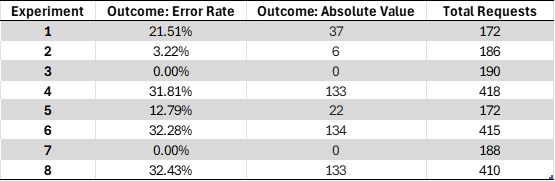
\includegraphics[width=0.8\textwidth]{media/factorial_outcome_per_y_plus_totrequests.png}
    \caption{Experiment Results and Total Number of Requests per Experiment.}
    \label{fig:results_totrequests}
\end{figure}

The factorial analysis results for each factor change, depending on the outcome being considered. Please consult the results in Figure \ref{fig:factors_effects}.

\begin{figure}[H]
    \centering
    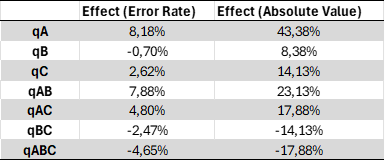
\includegraphics[width=0.5\textwidth]{media/Effects_Factors.png} \caption{Effects of each Factor, considering the different outcomes.}
    \label{fig:factors_effects}
\end{figure}

It is possible to assess that the effect of the factors changes in magnitude, depending on the outcome being considered, and factor B also changes in sign (or its impact).
Independently of the outcome being considered, factor A (Has On Demand Jobs) is
the one that contributes more towards requests failure. This means that a
higher value of Has On Demand Jobs is likely to lead to a higher failure number
(or rate) of requests. Other factors that contribute to the failure of requests are,
in descending order, interaction AB (Dkron Servers), interaction AC
(Dkron Agents) and factor C (Memory). On the other hand, interaction BC (Concurrent)
helps mitigating the number or rate of failed request, as well as the interaction ABC.
Factor B is negligible when the outcome is expressed in rate.

Finally, from the metrics gathered through k6, the metric req\_duration provides the response
time. Without much consideration, but solely looking into the values, the response time shows to
tend to grow as we have more Dkron Servers. This was expected since there are more Servers working
in the consensus. This means that the reliability provided by Dkron is easily noticeable with small
increments - in my benchmark experiments 3 to 7 Servers. However, due to time constraints, I
could not finish the response time analysis to provide a more in-dept conclusion.

\section{Conclusion}
\label{conclusion}

From the analysis of Dkron, the major assumption could be concluded when looking at K6 response time
metric: that increasing the amount of Dkron Servers increases response time. This is due
to the nature of the reliability characteristic supported by Dkron Servers, increasing crosstalk.

At the beginning of the analysis I was curious to understand the behavior of Dkron when
in high stress. It seems to handle relatively when, i.e., although the nodes become unstable,
Dkron is still able to respond to incoming requests and also execute the existing jobs. Nevertheless,
nodes crashed a lot due to high memory and cpu usage as I observed in K9 during the benchmark.

Other particularity that I observed is that, at most, 2 Servers were at 100\% cpu utilization, while
the other peers were relatively stable. It seems the Raft leader has a load a lot higher than its
peers, making Dkron leaders vulnerable to crashed, requiring frequent new leader elections.

In the end, Dkron shows to provide reliability through Dkron Servers, while providing performance gains
from Dkron Agents. Unfortunately it seemed dkron helm chart is not stable and the agent's template has bugs,
limiting me to either 0 or 1 agent.

%MEMORY LIMIT NOTES: although no memory heavy jobs are done, memory usage was very high (raft?)

\subsection{Limitations}
Deploying Dkron with helm proved to be challenging. Documentation is lacking, and
it seems there is no stable helm chart for dkron. Additionally, during bug fixing and deployment,
I was left with the idea that \href{https://github.com/distribworks/dkron/issues?q=helm}{a lot more other developers face their own
unexpected issues with dkron's helm chart}.

\section{Annexes}



\subsection{Metrics Visualisation}
The following Figures provide some visualisations about each experiment. All plots have the same x-axis order: NOs3a0-250-1NO, NOs3a0-500-2YES, NOs3a1-500-1NO,  YESs3a1-250-2NO, NOs7a1-250-1YES, YESs7a1-500-2YES,  YESs7a0-500-1NO, NOs7a0-250-2NO. This corresponds to the following experiment order: 2, 7, 3, 6, 1, 8, 4, 5.

\begin{figure}[H]
    \centering
    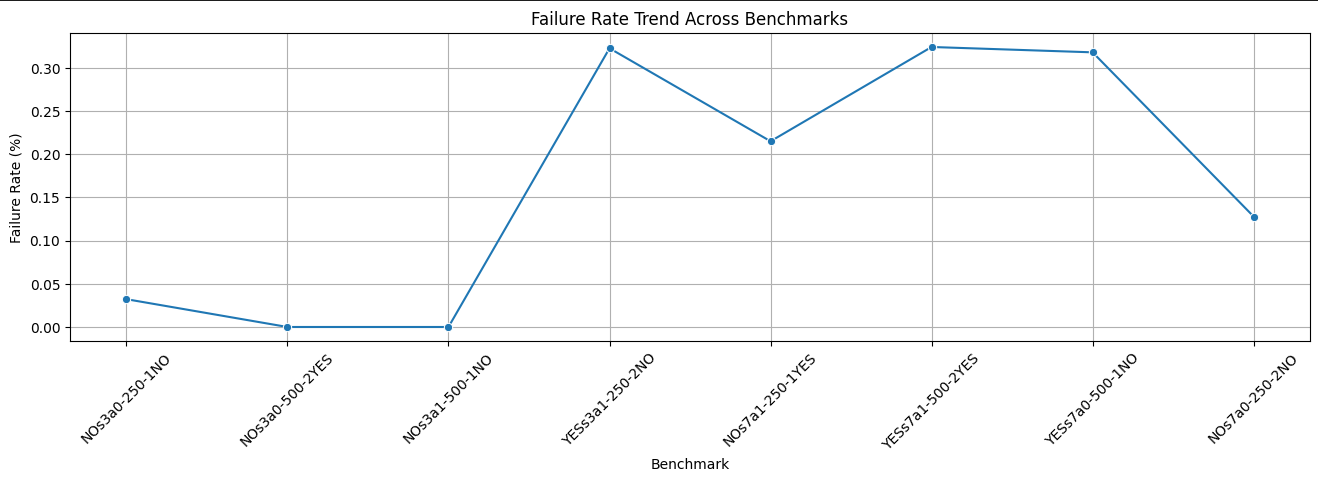
\includegraphics[width=1\textwidth]{media/FailureRate_trend.png} \caption{Failure Rate Trend Across Benchmarks}
    \label{fig:aaa}
\end{figure}

\begin{figure}[H]
    \centering
    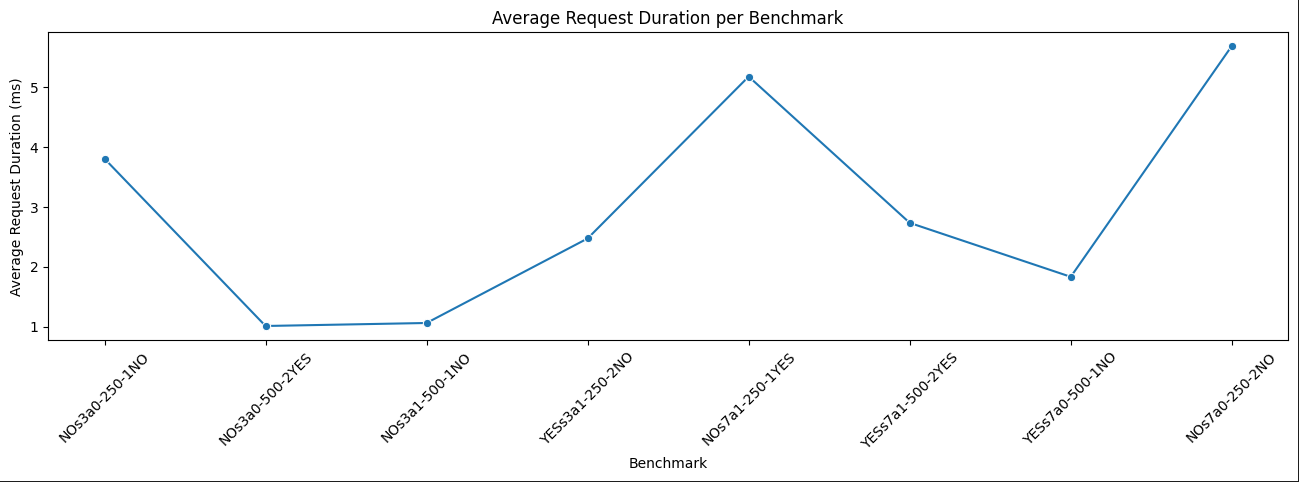
\includegraphics[width=1\textwidth]{media/Avg_req_duration.png} \caption{Average Request Duration Per Benchmark}
    \label{fig:bb}
\end{figure}

\begin{figure}[H]
    \centering
    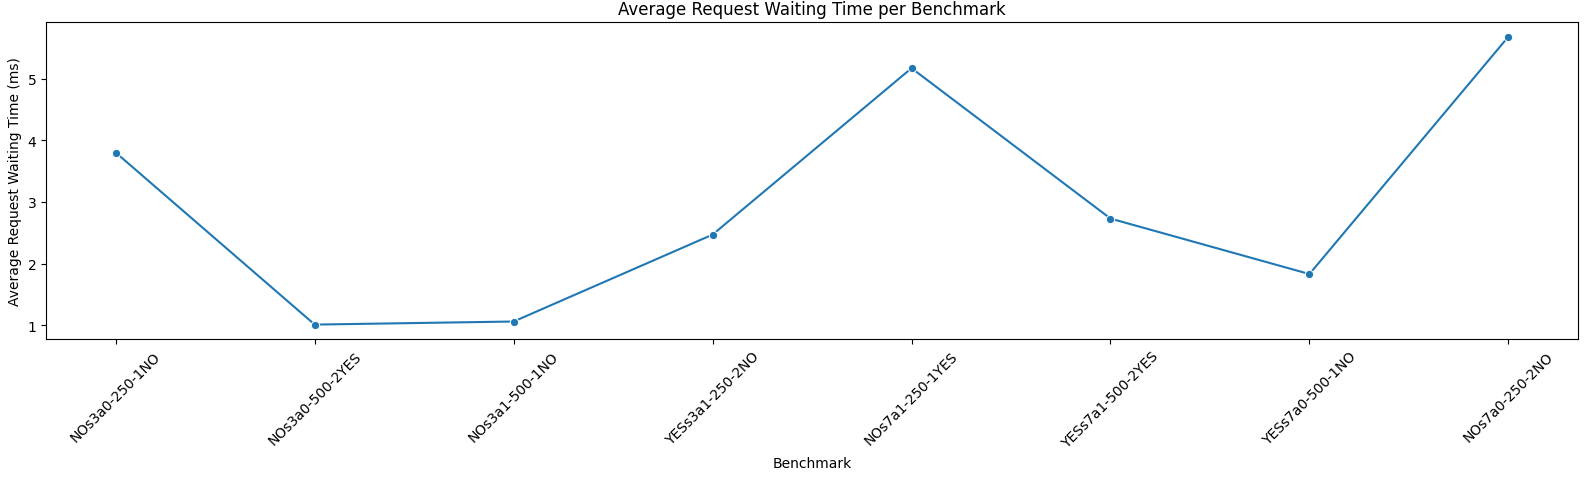
\includegraphics[width=1\textwidth]{media/Avg_req_waitingtime.png} \caption{Average Request Waiting Time Per Benchmark}
    \label{fig:cc}
\end{figure}

\begin{figure}[H]
    \centering
    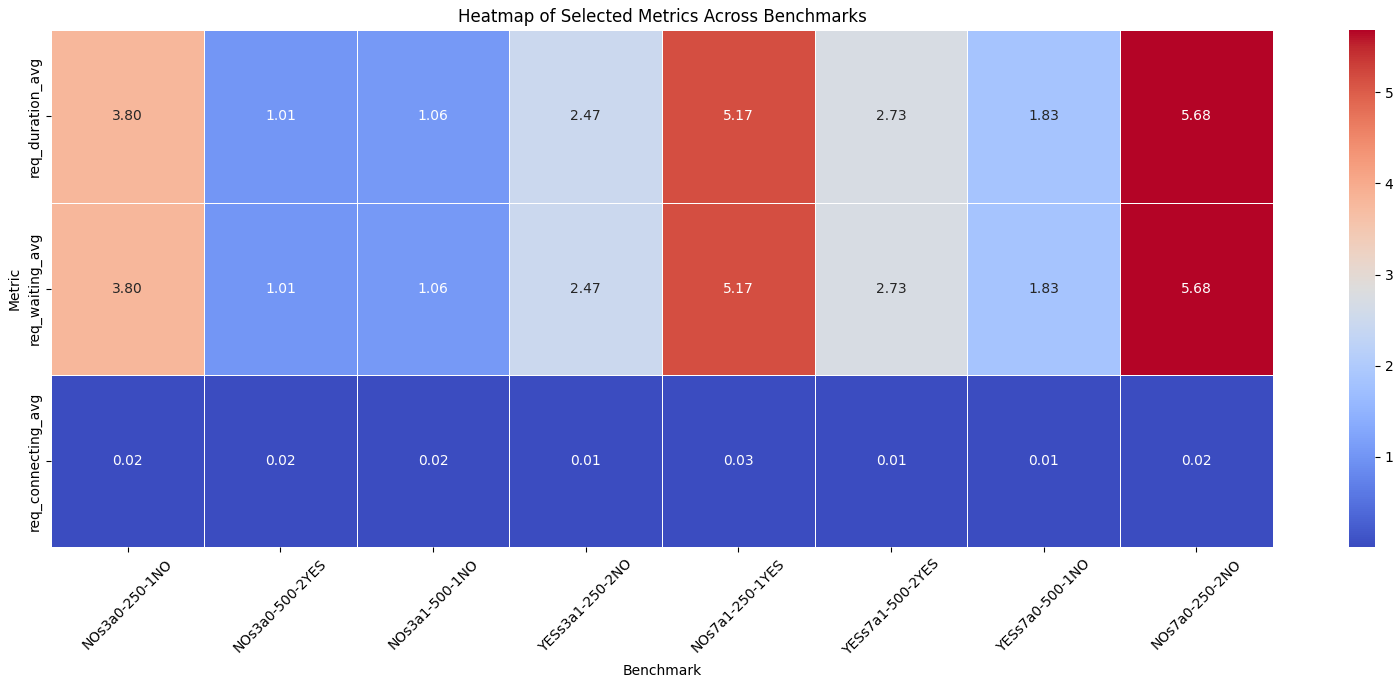
\includegraphics[width=1\textwidth]{media/heatmap_avgConnect_avgWait_avgDuration.png} \caption{HeatMap of selected metrics}
    \label{fig:fddd}
\end{figure}

\subsection{Factorial Analysis}
Figure \ref{fig:factorsdomain} provides the domains of the factors under analysis and that were used to build the benchmarks.

\begin{figure}[H]
    \centering
    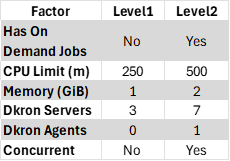
\includegraphics[width=0.3\textwidth]{media/FactorAnalysis_DomainFactors.png}
    \caption{Domain of the Factors.}
    \label{fig:factorsdomain}
\end{figure}

Figure \ref{fig:fulloriginalfactors} provides the sign table with the original values of each factor, allowing for a complete overview of each benchmark setup.

\begin{figure}[H]
    \centering
    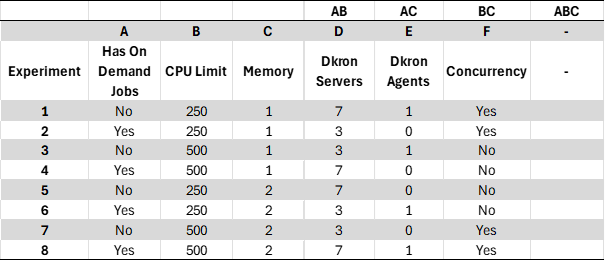
\includegraphics[width=0.8\textwidth]{media/FullFactorTable_OriginalFactors.png}
    \caption{Sign Table with Values.}
    \label{fig:fulloriginalfactors}
\end{figure}

\begin{figure}[H]
    \centering
    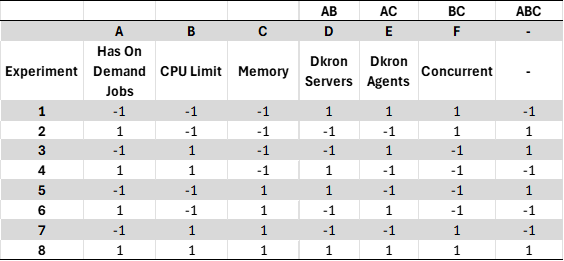
\includegraphics[width=0.8\textwidth]{media/FullFactorTable_onesminusones.png}
    \caption{Sign Table.}
    \label{fig:fullconvertedoriginalfactors}
\end{figure}


% ---- Bibliography ----
%
% BibTeX users should specify bibliography style 'splncs04'.
% References will then be sorted and formatted in the correct style.
%
% \bibliographystyle{splncs04}
% \bibliography{mybibliography}
%
\begin{thebibliography}{8}

\bibitem{mm2024}
Matos, M.: IST - Large Scale Systems Engineering - Class slides
Lisbon (2024)

\bibitem{dkron}
https://dkron.io/docs/intro
\bibitem{dkron2}
https://k6.io/docs/
\bibitem{dkron3}
https://helm.sh/docs/
\bibitem{dkron4}
https://kubernetes.io/docs/home/
\end{thebibliography}
\end{document}
